\section{Design}


\subsection{Transaction Sizes}

Key points: transactions have limited size, both in space and time. A
transaction cannot take too many instructions, nor have too many memory
accesses. Of course, we're designing under an assumption about how transactions
will work... they may turn out differently. So we're designing pessimistically.

num memory accesses matter more than number of instructions, but the total length
matters too.

We can also optimize certain parts of the code with Os and other parts with
O2/3.













\begin{figure}
\centering
\hspace*{-0.3in}
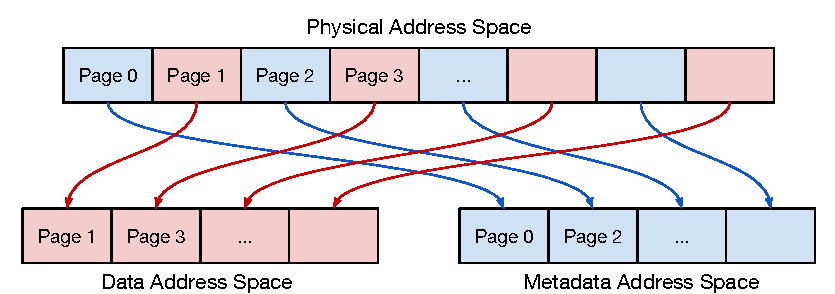
\includegraphics[width=88mm]{fig/addrspace}
\caption{Stuff.}
\label{fig:addrspace}
\end{figure}

\begin{figure}
\centering
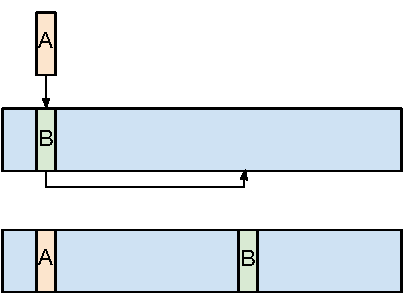
\includegraphics[width=70mm,height=50mm]{fig/cuckoo_insert}
\caption{Stuff.}
\label{fig:insert}
\end{figure}

\begin{figure}
\centering
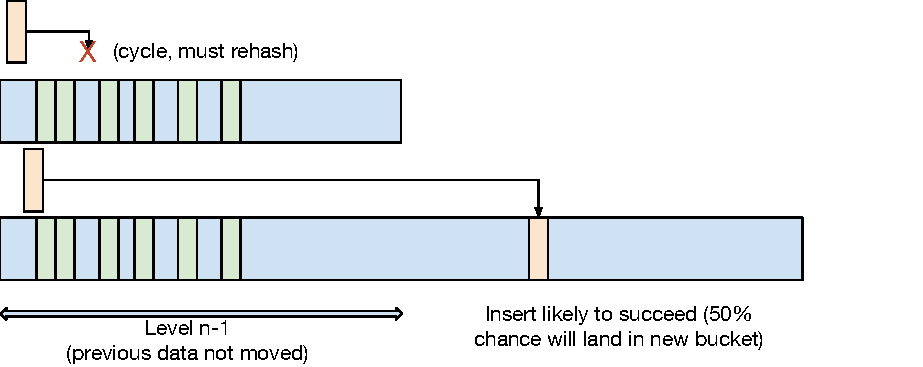
\includegraphics[width=100mm]{fig/cuckoo_rehash}
\caption{Stuff.}
\label{fig:rehash}
\end{figure}

